% Created 2019-09-05 jeu. 19:17
% Intended LaTeX compiler: pdflatex
\documentclass[presentation]{beamer}
\usepackage[utf8]{inputenc}
\usepackage[T1]{fontenc}
\usepackage{graphicx}
\usepackage{grffile}
\usepackage{longtable}
\usepackage{wrapfig}
\usepackage{rotating}
\usepackage[normalem]{ulem}
\usepackage{amsmath}
\usepackage{textcomp}
\usepackage{amssymb}
\usepackage{capt-of}
\usepackage{hyperref}
\RequirePackage{fancyvrb}
\DefineVerbatimEnvironment{verbatim}{Verbatim}{fontsize=\scriptsize}
\usetheme{default}
\author{Laurent Garnier}
\date{\today}
\title{Feuille de route pour créer un smart contract}
\hypersetup{
 pdfauthor={Laurent Garnier},
 pdftitle={Feuille de route pour créer un smart contract},
 pdfkeywords={},
 pdfsubject={},
 pdfcreator={Emacs 26.2 (Org mode 9.1.9)}, 
 pdflang={English}}
\begin{document}

\maketitle
\begin{frame}{Outline}
\tableofcontents
\end{frame}


\begin{frame}[fragile,label={sec:orgee05c55}]{Structure générale du dossier}
 Dans tout dossier chaincode il doit y avoir :
\begin{itemize}
\item un fichier nommé \texttt{chaincode.yaml}
\item un dossier \texttt{src}
\item dans le dossier \texttt{src} il doit y avoir :
\begin{enumerate}
\item Le code source \texttt{nom\_du\_fichier.go}
\item L'API de description \texttt{openapi.yaml}
\end{enumerate}
\end{itemize}

Voir la figure ci-dessous :

\begin{center}
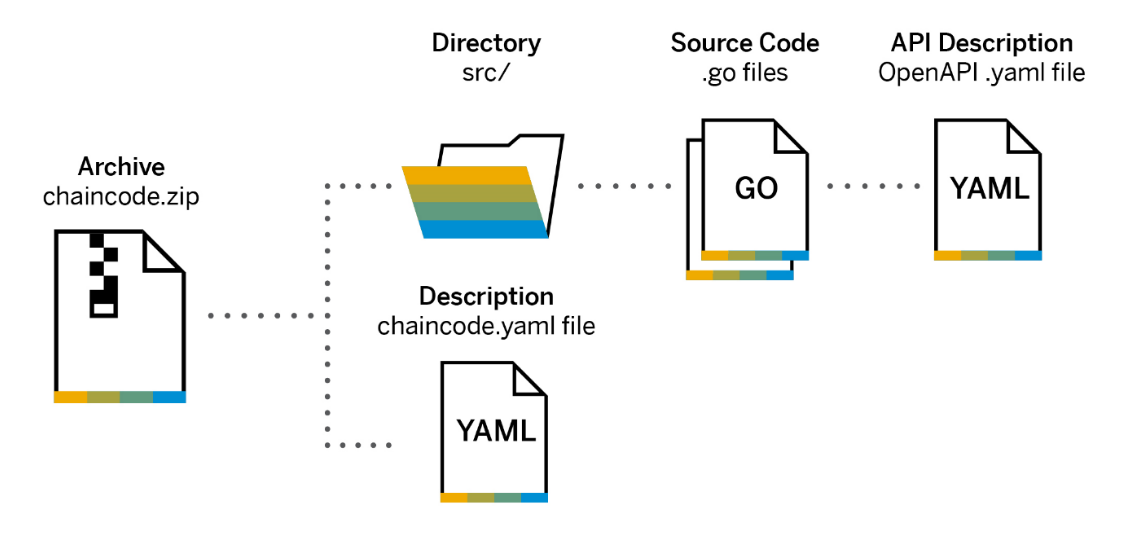
\includegraphics[width=.9\linewidth]{./chaincode_dir_struct.png}
\end{center}
\end{frame}

\begin{frame}[fragile,label={sec:org5ddcde9}]{Le fichier \texttt{chaincode.yaml}}
 Dans ce fichier nous fournirons les méta-données de notre chaincode.

Les balises Id et Version sont importantes ici. 

Chaque fois qu'un chaincode est appelé, soit depuis une API REST soit depuis un autre chaincode, l'identifiant (ID) 
du chaincode doit être connu. 

Cet ID doit aussi être fourni lorsque le chaincode est déployé.

Nous recommandons de spécifier tous les IDs de chaincode dans le format DNS inverse, comme pour les classes Java.

Par exemple, l'Id de notre chaincode est \texttt{blockchain-example-chaincode\_test}.

Cette syntaxe pour les IDs de chaincode : caractères alphanumérique et les tirets - et \_.

De la même manière, chaque chaincode se voit attribué un numéro de version.

Puisqu'un chaincode est déployé "pour toujours" sur la blockchain et ne peut être effacé, pour remplacer 
un chaincode on ré-utilise sont numéro de version.

Durant le déploiement, le numéro de version doit être disponible. 
\end{frame}

\begin{frame}[fragile,label={sec:org4c2ec44}]{Code du fichier \texttt{chaincode.yaml}}
 \begin{verbatim}
# THIS SAMPLE CODE MAY BE USED SOLELY AS PART OF A TEST 
# BLOCKCHAIN SERVICE (THE "SERVICE") AND IN ACCORDANCE 
# WITH THE TERMS OF THE AGREEMENT FOR THE SERVICE.
# THIS SAMPLE CODE PROVIDED "AS IS", WITHOUT ANY WARRANTY, 
# ESCROW, TRAINING, MAINTENANCE, OR SERVICE OBLIGATIONS 
# WHATSOEVER ON THE PART OF ALMERYS/BE|YS.

Id:       blockchain-example-chaincode_test
Version:  1
\end{verbatim}
\end{frame}

\begin{frame}[fragile,label={sec:org39e3864}]{Création du fichier de description API}
 ALMERYS/BE|YS fournit une porte d'entrée qui expose toutes les fonctions chaincode comme des APIs REST normales.

Vous pouvez accomplir cela en fournissant une description OpenAPI de l'API REST qui est liée aux fonctions du chaincode.

Vous faites cela avec le document YAML qui est écrit avec le chaincode en golang.

Le document YAML décrit exactement comment chaque fonction peut accédée via un appel REST, quels paramètres sont disponibles
et comment les paramètres doivent être transmis au chaincode.

Dans le dossier \texttt{src} créer un fichier \texttt{hello\_world.yaml} :
\end{frame}

\begin{frame}[fragile,label={sec:org2999f97}]{Code du fichier \texttt{hello\_world.yaml}}
 \begin{verbatim}
swagger: "2.0"
info:
  description: |
    The Hello World! chain code shows the first steps 
    in developing a chaincode that can read/write 
    strings onto the blockchain and can expose these 
    functions as REST API. 
    THIS SAMPLE CODE MAY BE USED SOLELY AS PART OF 
    THE TEST AND EVALUATION OF THE ALMERYS/BE|YS 
    BLOCKCHAIN SERVICE (THE "SERVICE") AND IN 
    ACCORDANCE WITH THE AGREEMENT FOR THE SERVICE. 
    THIS SAMPLE CODE PROVIDED "AS IS", WITHOUT ANY 
    WARRANTY, ESCROW, TRAINING, MAINTENANCE, OR 
    SERVICE OBLIGATIONS WHATSOEVER ON THE PART OF 
    ALMERYS/BE|YS.
  version: "1.0"
  title: "Hello World!"
\end{verbatim}
\end{frame}

\begin{frame}[label={sec:org1b3c659}]{Création du fichier du code source (en Golang)}
Lors du développement d'un chaincode, l'étape suivante est d'écrire le programme 
GO lui-même (ce qui est notre chaincode).

Dans le programme, il peut y avoir un nombre quelconque de fonctions, chaque 
fonction ayant un nombre quelconque de paramètres "non nommés".

L'appelant de toute fonction doit connaître le nom de la fonction et de la séquence 
exacte de paramètres. 

Dans les configurations Hyperledger Fabric standards, l'accès au chaincode se fait 
uniquement via un SDK ce qui requiert un accès du chaincode au HTTPS/gRPC.
\end{frame}

\begin{frame}[fragile,label={sec:org202beb8}]{Code du fichier \texttt{hello\_world.go} :}
 \begin{verbatim}
// DISCLAIMER:
// THIS SAMPLE CODE MAY BE USED SOLELY AS PART OF THE TEST 
// AND EVALUATION OF THE ALMERYS/BE|YS BLOCKCHAIN SERVICE 
// (THE "SERVICE") AND IN ACCORDANCE WITH THE TERMS OF THE 
// AGREEMENT FOR THE SERVICE. THIS SAMPLE CODE PROVIDED 
// "AS IS", WITHOUT ANY WARRANTY, ESCROW, TRAINING, 
// MAINTENANCE, OR SERVICE OBLIGATIONS WHATSOEVER ON THE 
// PART OF ALMERYS/BE|YS.
\end{verbatim}
\end{frame}

\begin{frame}[fragile,label={sec:orgb76f664}]{Comprendre le fichier de description API}
 Le fichier de description API \texttt{hello\_world.yaml} est utilisé pour décrire l'interface
HTTP exacte pour le chaincode.

C'est important de comprendre que le fichier \texttt{.yaml} est ensuite utilisé dans deux 
contextes différents : 
\begin{itemize}
\item Pour générer la page de test API depuis laquelle les APIs de chaincode peuvent 
être testées directement
\item La passerelle d'API utilise des aspects spécifiques du fichier YAML pour décider 
de la méthode d'extraction des paramètres de la requête HTTP entrante. Ensuite, 
ils associent ces éléments à une fonction du chaincode à appeler.
\end{itemize}
\end{frame}
\begin{frame}[fragile,label={sec:org13058c6}]{Comprendre la correspondance verbes HTTP et appels de chaincode}
 Un ensemble riche de verbes HTTP est utilisé de manière spécifique pour que 
les appels REST imitent les opérations CRUD (Create Read Update Delete) typiques
des bases de données.

Du côté Hyperledger Fabric, les fonctions chaincode peuvent être appelées comme suit : 

\begin{itemize}
\item Par un appel \texttt{Invoke} qui écrit une transaction avec des ensembles lecture/écriture 
dans la blockchain
\item Par un appel \texttt{Query} pour un type de fonction en lecture seule
\end{itemize}


Pour toutes les demandes HTTP entrantes, chaque verbe HTTP spécifique correspond à un 
appel Invoque ou Query de Hyperledger Fabric.

Dans cet exemple de chaincode, nous utiliserons des appels POST et GET.
\end{frame}

\begin{frame}[label={sec:org400ca83}]{Tableau des correspondances HTTP/Chaincode}
\begin{center}
\begin{tabular}{llll}
Verbe HTTP & Action type & Correspond à & Effet sur la Blockchain\\
\hline
POST & Créer & Invoke & Ecrit une transaction\\
\hline
GET & Lire & Query & Aucun\\
\end{tabular}
\end{center}
\end{frame}


\begin{frame}[fragile,label={sec:org718930f}]{Comprendre les chemins de chaincode}
 La section des chemins de chaincode est utilisée pour définir une définition 
enrichie de l'API basée sur REST et toutes les fonctionnalités de Swagger 
peuvent être utilisées pour décrire l'API. Deux cas spéciaux s'appliquent : 

\begin{itemize}
\item Pour chaque chemin, vous devez préciser l'\texttt{operationId}. C'est le nom de direct de la 
fonction chaincode qui doit être appelée pour ce chemin.
\item Pour les paramètres, les cinq emplacements de paramètres sont pris en charge. Les paramètres
peuvent être \texttt{path}, \texttt{query}, \texttt{header}, \texttt{form}, ou \texttt{body}. Pour les types de paramètres, 
vous pouvez utiliser uniquement des paramètres simples qui peuvent être mis en correspondance
avec des type de chaîne de caractères en entrée de chaincode. Les types acceptés sont : 
\texttt{string}, \texttt{number}, \texttt{integer}, \texttt{boolean}, et \texttt{file}.
\end{itemize}
\end{frame}

\begin{frame}[fragile,label={sec:org3a3de04}]{Définir le chemin du chaincode de \texttt{POST}}
 Pour définir le chemin d'accès au chaincode (utilisé pour appeler le chaincode), 
ouvrir le fichier \texttt{hello\_world.yaml} avec un éditeur de texte et copiez-collez les lignes suivantes :
\end{frame}

\begin{frame}[fragile,label={sec:orgc414a8b}]{Code du fichier \texttt{hello\_world.yaml}}
 \begin{verbatim}
consumes:
  - application/x-www-form-urlencoded

paths:

  /{id}:

    post:
      operationId: write
      summary: Write a text (once) by ID
      parameters:
      - name: id
	in: path
	required: true
	type: string
      - name: text
	in: formData
	required: true
	type: string
      responses:
	200:
	  description: Text Written
	500:
	  description: Failed
\end{verbatim}
\end{frame}

\begin{frame}[fragile,label={sec:org221c824}]{Explications}
 Ce chemin de publication (\texttt{POST}) inclut la fonction write (\texttt{operationID: write}), deux paramètres pouvant être écrits 
(\texttt{id} et \texttt{text}) et deux codes de réponse (200 pour la réussite de la publication et 500 pour l'échec).

Notez que cet exemple inclut également la section \texttt{consumes}. 

Ceci définit les types de contenu par défaut qui seront acceptés pour tous les appels d'API, s'ils ne sont pas définis 
spécifiquement. Par défaut, il doit être défini sur \texttt{application/x-www-form-urlencoded} pour signaler que les demandes 
HTTP entrantes auront des paramètres au format nom / valeur.
\end{frame}
\begin{frame}[fragile,label={sec:org07bd5da}]{Définir le chemin \texttt{GET}}
 Pour définir le chemin de chaincode \texttt{GET} (utilisé pour interroger le chaincode), 
copiez et collez les lignes suivantes sous le code précédent :
\end{frame}



\begin{frame}[fragile,label={sec:orgb8e01f0}]{Code du fichier \texttt{hello\_world.yaml}}
 \begin{verbatim}
get:
     operationId: read
     summary: Read text by ID
     parameters:
     - name: id
       in: path
       required: true
       type: string
       produces:
     - text/plain
     responses:
       200:
	 description: OK
       500:
	 description: Failed
\end{verbatim}
\end{frame}
\begin{frame}[fragile,label={sec:org265b656}]{Explications}
 Ce chemin pour \texttt{GET} comprend les fonctions de lecture (\texttt{operationID: read}), 
un paramètre à lire (\texttt{id}) et deux codes de réponse (200 pour une lecture 
réussie et 500 pour un échec de lecture).
\end{frame}
\begin{frame}[fragile,label={sec:org07c3483}]{Valider le \texttt{hello\_world.yaml} avec Swagger.io}
 Ouvrir un navigateur web et naviguer jusqu'à l'éditeur \href{https://editor.swagger.io/}{Swagger.io}

Cliquer sur File > Clear Editor

\begin{center}
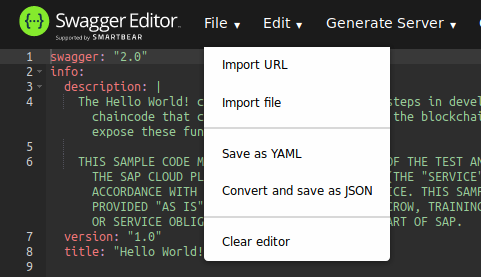
\includegraphics[width=.9\linewidth]{./swagger_file_clear.png}
\end{center}

Puis copier le code du fichier \texttt{hello\_world.yaml} à l'intérieur
\end{frame}

\begin{frame}[label={sec:orgc388d89}]{Swagger complet}
\begin{center}
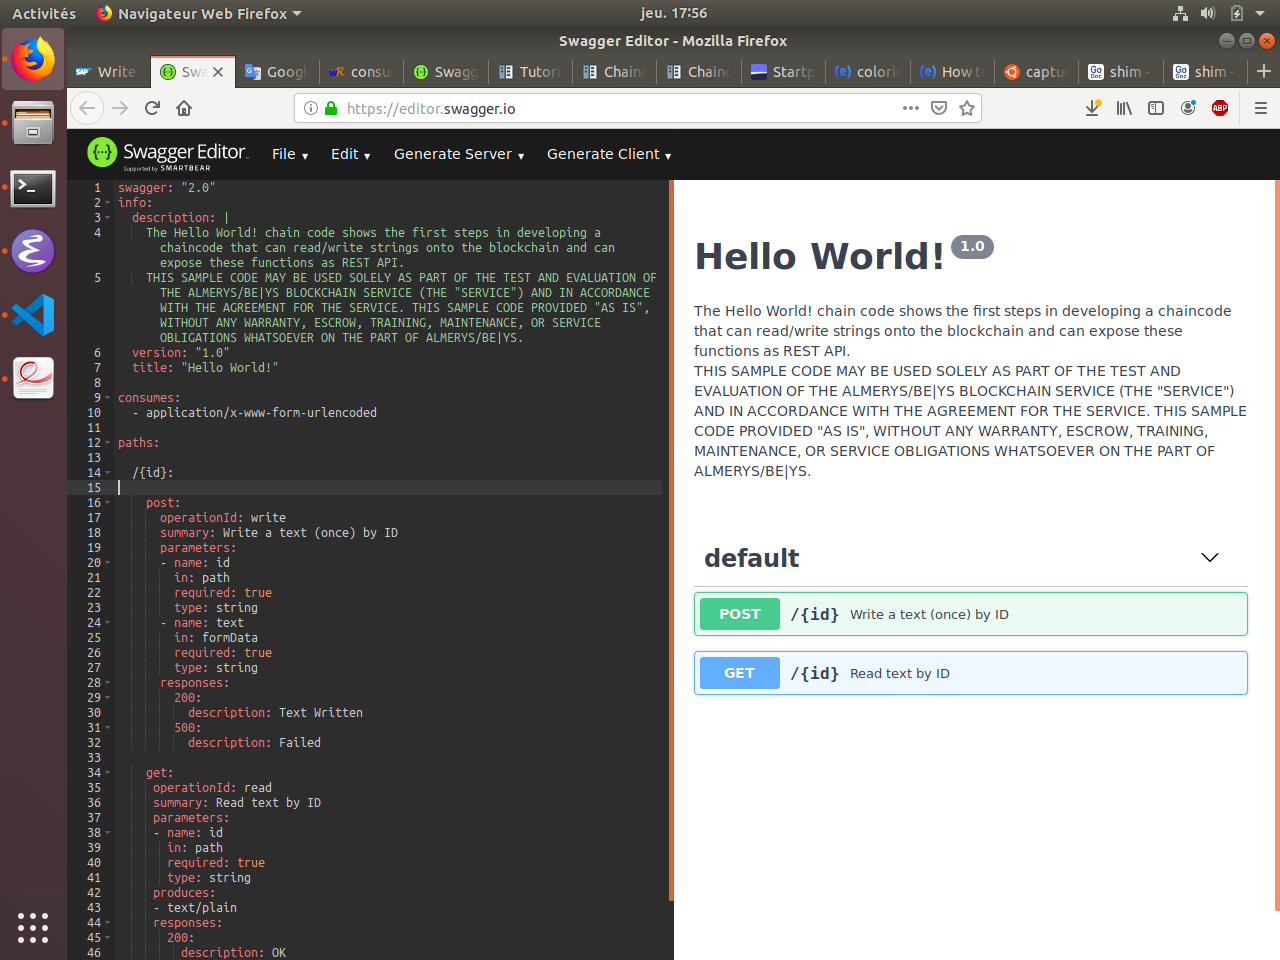
\includegraphics[width=.9\linewidth]{./swagger_complete.png}
\end{center}
\end{frame}
\begin{frame}[label={sec:org76c9c46}]{Comprendre les avantages des outils de développement de chaincode}
Un chaincode est un programme développé en utilisant le langage de 
programmation GO. Pour le cycle de développement, il est plus efficace
de pouvoir vérifier la syntaxe des programmes GO avant de les télécharger
et de les déployer sur le noeud Hyperledger Fabric. Vous pouvez facilement
le faire avec une installation minimale.
\end{frame}

\begin{frame}[fragile,label={sec:org2f34247}]{Installer Git et Golang}
 \begin{block}{Télécharger}
\begin{itemize}
\item Télécharger Git : \url{https://git-scm.com/downloads}
\item Télécharger Go : \url{https://golang.org/dl/}
\end{itemize}
\end{block}
\begin{block}{Valider}
Pour valider les installations, ouvrir un terminal et taper :
\begin{itemize}
\item \texttt{git}
\item \texttt{go}
\end{itemize}

Dans les deux cas des documentations s'afficheront à l'écran
\end{block}
\end{frame}
\begin{frame}[fragile,label={sec:org1a08414}]{Installer les paquets Hyperledger}
 Utilisons \texttt{go} et \texttt{git} :

\begin{verbatim}
go get github.com/hyperledger/fabric/common/util

go get github.com/hyperledger/fabric/core/chaincode/shim

go get github.com/hyperledger/fabric/protos/peer
\end{verbatim}
\end{frame}

\begin{frame}[fragile,label={sec:org3c91350}]{Création du \texttt{package main}}
 Le chaincode de Hyperledger Fabric est essentiellement un morceau de code exécuté sur un nœud homologue. 

Lors de la création de ce code, vous utiliserez le package «main» pour en faire un programme exécutable. 

Ce paquetage «main» indique au compilateur de Go, installé dans le tutoriel précédent, que le paquet doit 
être compilé en tant que programme exécutable au lieu d’une bibliothèque partagée (utilisée pour les 
morceaux de code réutilisables).

La fonction principale du paquet «main» sera le point d’entrée de notre programme exécutable. 

Ceci est utilisé pour créer un binaire avec go build.

Ouvrez votre fichier \texttt{hello\_world.go}, copiez et collez le texte ci-dessous sous l'avertissement :

\begin{verbatim}
package main
\end{verbatim}
\end{frame}
\begin{frame}[fragile,label={sec:org829c0a2}]{Importer des \texttt{packages}}
 Dans Go, les fichiers source sont organisés dans des répertoires système appelés packages. 

Ceux-ci permettent la réutilisation de code dans les applications Go. 

Le mot clé "import" est utilisé pour importer un package. 

Nous pouvons télécharger et installer des packages Go tiers en utilisant la commande \texttt{go get}. 

La commande \texttt{go get} va extraire les packages du référentiel source et les placer sur l'emplacement \texttt{GOPATH}.

Ouvrez votre fichier \texttt{hello\_world.go}, copiez et collez ce qui suit sous le paquet principal :
\end{frame}
\begin{frame}[fragile,label={sec:orgf985e17}]{Code du fichier \texttt{hello\_world.go}}
 \begin{verbatim}
package main {
  import (
	"github.com/hyperledger/fabric/core/chaincode/shim"
	"github.com/hyperledger/fabric/protos/peer"
  )
}
\end{verbatim}
\end{frame}
\begin{frame}[fragile,label={sec:org2a0e702}]{Définir un chaincode}
 Lorsque le code de chaîne est démarré sur un nœud homologue, la fonction principale est exécutée. 

Le chaincode est ensuite démarré avec \texttt{shim.Start}, qui attend une structure qui implémente l'interface \texttt{shim.Chaincode}.

Ouvrez votre fichier \texttt{hello\_world.go}, copiez et collez le type et les fonctions principales sous les packages d'importation :

\begin{verbatim}
type Chaincode struct {
}

func main() {
     shim.Start(new(Chaincode))
}
\end{verbatim}
\end{frame}
\begin{frame}[fragile,label={sec:orge4c4224}]{Implémentation d'une interface chaincode}
 Tout chaincode a besoin de l'interface suivante : 

\begin{verbatim}
type Chaincode interface {
  // Init is called during Instantiate transaction after 
  // the chaincode container
  // has been established for the first time, allowing 
  // the chaincode to initialize its internal data
  Init(stub ChaincodeStubInterface) peer.Response

  // Invoke is called to update or query the ledger 
  // in a proposal transaction.
  // Updated state variables are not committed to 
  // the ledger until the transaction is committed.
  Invoke(stub ChaincodeStubInterface) peer.Response
}
\end{verbatim}
\end{frame}
\begin{frame}[fragile,label={sec:org99aa9ad}]{Explications}
 Lorsque vous instanciez ou mettez à niveau un code de chaîne, la fonction Init de ce dernier est exécutée. 

Vous pouvez l'utiliser pour initialiser des valeurs sur le grand livre.

Lorsque vous appelez ou interrogez un code de chaîne, la fonction Invoke de ce dernier est exécutée. 

Vous pouvez l'utiliser pour mettre à jour ou interroger le grand livre.

REMARQUE: vous trouverez des informations supplémentaires sur cette interface à l'adresse \href{https://godoc.org/github.com/hyperledger/fabric/core/chaincode/shim\#Chaincode}{GoDoc.org}.

Les fonctions Init et Invoke sont toutes deux appelées à l’aide de l’\href{https://godoc.org/github.com/hyperledger/fabric/core/chaincode/shim\#ChaincodeStubInterface}{interface stub}, qui permet 
d’accéder aux paramètres de transaction et de modifier le grand livre.

Ouvrez votre fichier \texttt{hello\_world.go}, copiez et collez les fonctions init et invoke sous les packages d'importation :
\end{frame}
\begin{frame}[fragile,label={sec:orgb34e5a7}]{Code à ajouter au fichier \texttt{hello\_world.go}}
 \begin{verbatim}
// Init is called during Instantiate transaction.
func (ptr *Chaincode) Init(stub shim.ChaincodeStubInterface) peer.Response {
	return shim.Success(nil)
}

// Invoke is called to update or query the ledger in a proposal transaction.
func (ptr *Chaincode) Invoke(stub shim.ChaincodeStubInterface) peer.Response {
	return shim.Error("Not yet implemented!")
}
\end{verbatim}
\end{frame}
\begin{frame}[label={sec:orgcc701c5}]{Ajouter des fonctions au chaincode}
\begin{center}
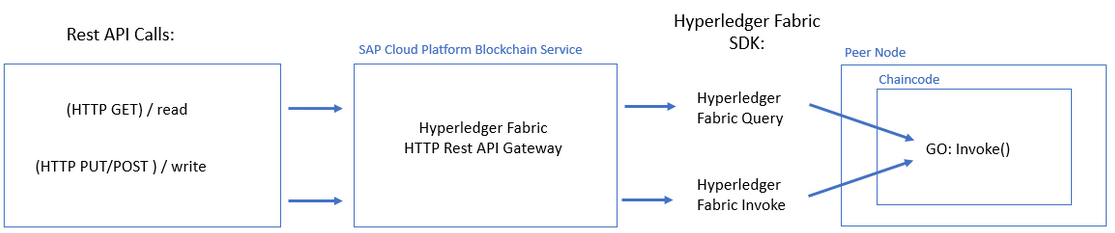
\includegraphics[width=.9\linewidth]{./rest_api_calls.png}
\end{center}

Dans Hyperledger Fabric, nous devons faire la distinction entre les différents contextes dans lesquels
le mot «Invoke» est utilisé. 
Dans Fabric, plus précisément dans le SDK utilisé pour accéder à toutes les fonctionnalités de Fabric, 
il existe le concept / accès de Invoke à Query. 
Un appel à la fonctionnalité Invoke au niveau du SDK Fabric est une opération 
d'écriture dans la blockchain sous-jacente. 
Après l'appel, toutes les mises à jour sont validées dans la blockchain. 
Cependant, un appel à la fonctionnalité Query est en réalité une opération de lecture sur la blockchain, 
qui ne renvoie que des informations.
\end{frame}

\begin{frame}[fragile,label={sec:org624ce69}]{Exlications [1/2]}
 Étant donné les concepts Invoke et Query dans Fabric (au niveau du SDK), 
le monde HTTP REST peut être mis en correspondance sur ces deux appels. 
En réalité, toutes les requêtes HTTP \texttt{GET} sont considérées comme des 
opérations de lecture et sont mises en correspondance sur un appel Query dans le SDK de Fabric. 
Tous les appels HTTP \texttt{POST} et \texttt{PUT} sont considérés comme des opérations d'écriture et sont
mis en correspondance sur l'appel Fabric Invoke.

Toutefois, les concept Invoke et Query sur le SDK de Fabric ne correspondent pas de façon biunivoque
dans le chaincode de Fabric. 
\end{frame}

\begin{frame}[fragile,label={sec:org020d50c}]{Explications [2/2]}
 Dans le chaincode, il n'y a qu'une seule fonction Invoke (implémentée dans le chaincode à l'aide du langage GO). 
Ainsi, dans le chaincode, il n'y a que des fonctionnalités de chaincode (également appelées fonctions), qui sont 
toutes accessibles via le point d'entrée central de la fonction Invoke (langage GO). 
Cette fonction GO Invoke ne sait en aucun cas si l'appel de l'extérieur était un Invoke (équivaut à écrire / valider) 
ou un Query (équivaut à une lecture). 
La fonction du chaincode doit simplement exécuter et renvoyer les réponses appropriées (correctes).

Lors de l'appel de chaincode via invoke ou query, la fonction Invoke du chaincode est exécutée. 

Pour accéder au nom de la fonction et aux arguments de l'appel, vous pouvez utiliser le \texttt{stub.GetFunctionAndParameters}. 
Vous pouvez ensuite utiliser le nom de la fonction pour appeler différentes fonctions.
\end{frame}

\begin{frame}[fragile,label={sec:org4e5d38c}]{Code de la fonction \texttt{Invoke}}
 \begin{verbatim}
func (ptr *Chaincode) Invoke(stub shim.ChaincodeStubInterface) peer.Response {
      function, args := stub.GetFunctionAndParameters()
      switch function {
	case "write":
	      return write(stub, args)  
	case "read":
	      return read(stub, args)
	default:
	      return shim.Error("unknown function")
      }
}
\end{verbatim}
\end{frame}
\begin{frame}[label={sec:org9ee9680}]{Explications [1/2]}
Dans notre exemple de code de chaîne, nous souhaitons mettre à jour notre fonction Invoke 
afin de différencier les actions, telles qu'écrire et lire. Nous faisons cela en créant 
deux nouvelles fonctions, intitulées écrire et lire. La fonction d'écriture vous permet 
d'écrire quelque chose dans le grand livre, alors que la fonction de lecture extrait des 
données et en fournit l'état.

Une fois que la fonction GO de Invoke () a identifié la fonctionnalité de code de chaîne 
appelée (Lecture ou Ecriture), elle appelle la fonction GO correspondante, en fournissant 
en tant que paramètres l'interface de stub et le tableau complet de chaînes, qui sont des 
paramètres d'entrée pour la fonction de code chaîne.

L'interface de module de remplacement est une interface de rappel qui peut être utilisée 
dans le code de chaîne pour accéder aux fonctionnalités de Fabric. Elle est décrite en 
détail dans la documentation de Fabric.
\end{frame}

\begin{frame}[label={sec:org3b6843d}]{Explications [2/2]}
Tous les paramètres de toute fonctionnalité de code de chaîne sont organisés en chaînes 
dans un tableau du code de chaîne. Il n'y a pas de contrôle sur le nombre de paramètres 
fournis, ni sur le type de chaque paramètre. Il appartient à la fonctionnalité de code 
de chaîne, en réalité à chaque fonction GO, de valider d’abord que le nombre et les 
types des paramètres d’entrée fournis correspondent, puis de décompresser et de convertir 
les chaînes en paramètres correspondants. Dans cet exemple, comme seuls les paramètres de 
chaîne sont utilisés, la seule vérification requise est de s'assurer que le nombre correct 
de paramètres a été fourni. De plus, tous les paramètres d'ID sont systématiquement remplacés 
par des minuscules, afin de garantir que la lecture et l'écriture fonctionneront toujours, 
indépendamment des chaînes d'identifiant fournies. (Notez que cela n’a pas à être fait, c’est
simplement un exemple de la façon dont les paramètres peuvent être transformés avec le chaincode 
avant d’être écrits dans le blockchain.)
\end{frame}
\begin{frame}[fragile,label={sec:orga252e1c}]{Code de la fonction \texttt{write}}
 \begin{verbatim}
// Write text by ID
func write(stub shim.ChaincodeStubInterface, args []string) peer.Response {

      if len(args) != 2 || len(args[0]) < 3 || len(args[1]) == 0 {
	      return shim.Error("Parameter Mismatch")
      }
      id := strings.ToLower(args[0])
      txt := args[1]

      if err := stub.PutState(id, []byte(txt)); err != nil {
	      return shim.Error(err.Error())
      }

      return shim.Success(nil)
}
\end{verbatim}
\end{frame}
\begin{frame}[label={sec:org6875754}]{Explications [1/3]}
La fonction write prend deux paramètres, à savoir l'ID de la chaîne et la valeur de chaîne elle-même. 
Un appel peut par exemple être écrit ("TXT001", "Hello World!"). 
La première étape de la fonction write consiste à vérifier que deux paramètres (de type chaîne) sont 
fournis, que le premier paramètre (ID) comporte au moins 3 caractères et que le second paramètre (la 
valeur du texte) est fourni (longueur supérieure à zéro).

Une fois les paramètres validés, nous extrayons les deux paramètres du tableau de chaînes (args [])
et les affectons à des variables GO locales. Habituellement, à cette étape, toutes les vérifications 
de type et les conversions supplémentaires sont effectuées, par exemple, la conversion de chaînes en 
entiers, etc., le cas échéant. Dans cet exemple, la seule manipulation de paramètre effectuée consiste 
à traduire l'ID en minuscule, afin de s'assurer qu'il est insensible à la casse.
\end{frame}

\begin{frame}[label={sec:orgc32be07}]{Explications [2/3]}
Dans l'étape suivante, la chaîne de texte doit être écrite dans la chaîne de blocs. 
La façon dont cela fonctionne, est que toutes les informations écrites dans la chaîne de blocs sont 
regroupées dans un blob et stockées sous une clé à l'aide de la méthode PutState sur l'interface de stub. 
Dans les applications complexes, la clé sera indexée sur l'objet métier et la charge utile sera une chaîne  
sérialisée (JSON) pour l'objet. 
Dans cet exemple, nous utilisons simplement l'ID directement en tant que clé et la valeur de texte 
directement en tant que charge utile. Ces deux paramètres sont utilisés comme entrée dans PutState. 
Le seul aspect mineur est que cette méthode attend un tableau d'octets ([] octets) en tant que paramètre 
d'entrée. 
Nous effectuons donc un transtypage en langage GO uniquement pour convertir la chaîne en tableau d'octets.
\end{frame}

\begin{frame}[label={sec:org2104449}]{Explications [3/3]}
Dans une dernière étape, nous retournons simplement un message de réussite.

Comment savons-nous / déterminons-nous que l'ID est le premier paramètre (args [0]) et que la valeur textuelle 
est le deuxième paramètre (args [1])? 

Ceci est appliqué et documenté dans l'interface HTTP REST correspondante (fichier YAML) qui décrit l'interface 
vers cette fonction. 

Là, deux paramètres ont été définis en tant qu'entrée dans l'appel HTTP REST / write et les paramètres sont 
transmis au code de chaîne dans exactement la séquence dans laquelle ils ont été définis dans le fichier YAML.
\end{frame}
\begin{frame}[fragile,label={sec:orgf0080d2}]{Code de la fonction \texttt{read}}
 \begin{verbatim}
// Read text by ID
func read(stub shim.ChaincodeStubInterface, args []string) peer.Response {

      if len(args) != 1 {
	      return shim.Error("Parameter Mismatch")
      }
      id := strings.ToLower(args[0])

      if value, err := stub.GetState(id); err == nil && value != nil {
	      return shim.Success(value)
      }

      return shim.Error("Not Found")
}
\end{verbatim}
\end{frame}

\begin{frame}[label={sec:org9ef61ca}]{Explications [1/2]}
La fonction de lecture est un peu plus simple. 

Il ne prend qu'un seul paramètre en entrée (l'ID de la chaîne à lire) et renvoie la valeur textuelle de la chaîne. 

Ce sera normalement appelé text = read ("TXT001"). 

Dans le premier, on vérifie qu'un seul paramètre est fourni. 

Notez que nous avons simplement ignoré la vérification de longueur ici, car nous allons valider l'ID implicitement 
un peu plus tard lors de la lecture de la blockchain.
\end{frame}

\begin{frame}[label={sec:org6f9e76c}]{Explications [2/2]}
Dans l'étape suivante, nous extrayons à nouveau l'ID en tant que variable GO du tableau de chaînes (args []).

La lecture de la blockchain est effectuée avec la méthode GetState. 

L'ID est fourni en tant que paramètre d'entrée et GetState renverra un tableau d'octets avec la valeur de blob 
correspondante dans la chaîne de blocs. Si nous réussissons (pas d'erreur et une valeur retournée), nous 
renverrons ce blob à l'appelant. Notez que l'appel Success prend également un tableau d'octets ([] byte) en 
tant que paramètre de retour, ce qui signifie que nous pouvons renvoyer directement l'objet blob récupéré, qui 
est notre valeur de texte. L'appelant (à l'extérieur) le convertira en une chaîne à renvoyer à l'appelant HTTP.

Si la lecture a échoué, par exemple parce que l'ID n'existe pas, un message d'erreur est renvoyé.
\end{frame}
\begin{frame}[fragile,label={sec:org9e2b86d}]{Comprendre les exigences de \texttt{packages} [1/2]}
 Lorsque le chaincode Hyperledger Fabric est prêt à être déployé, il doit être emballé dans une archive ZIP 
(sans exigences de nommage strictes). Cette archive zip doit inclure les fichiers suivants :

\begin{itemize}
\item manifeste \texttt{chaincode.yaml}
\item code GO de chaincode (\texttt{.go})
\item Description OpenAPI (\texttt{.yaml})
\end{itemize}


Le fichier \texttt{chaincode.yaml} doit porter exactement ce nom de fichier et doit être stocké dans le répertoire 
racine de l’archive ZIP.

En outre, il doit exister un dossier \texttt{/src} dans l’archive ZIP contenant les fichiers \texttt{.go} et \texttt{.yaml} qui 
représentent le code de chaîne. 

Vous n'êtes pas obligé de placer le code source du chaincode directement dans le dossier \texttt{/src}. 
\end{frame}

\begin{frame}[fragile,label={sec:org90d1a2d}]{Comprendre les exigences de \texttt{packages} [2/2]}
 Vous pouvez créer un chemin source plus profond (qui commence toujours par \texttt{/src}) dans l'archive ZIP, 
par exemple :

\texttt{/src/myChaincode/}.

Les fichiers \texttt{.go} et \texttt{.yaml} du chaincode doivent ensuite être stockés dans ce chemin source.

Si d'autres packages sont requis pour le chaincode, ils peuvent également être placés dans le 
dossier \texttt{/src} dans leurs propres sous-dossiers, en suivant l'approche du langage GO habituel 
pour la structuration du code source.
\end{frame}
\end{document}
